\section{免费办公用品}
\begin{figure}[H]
    \centering
    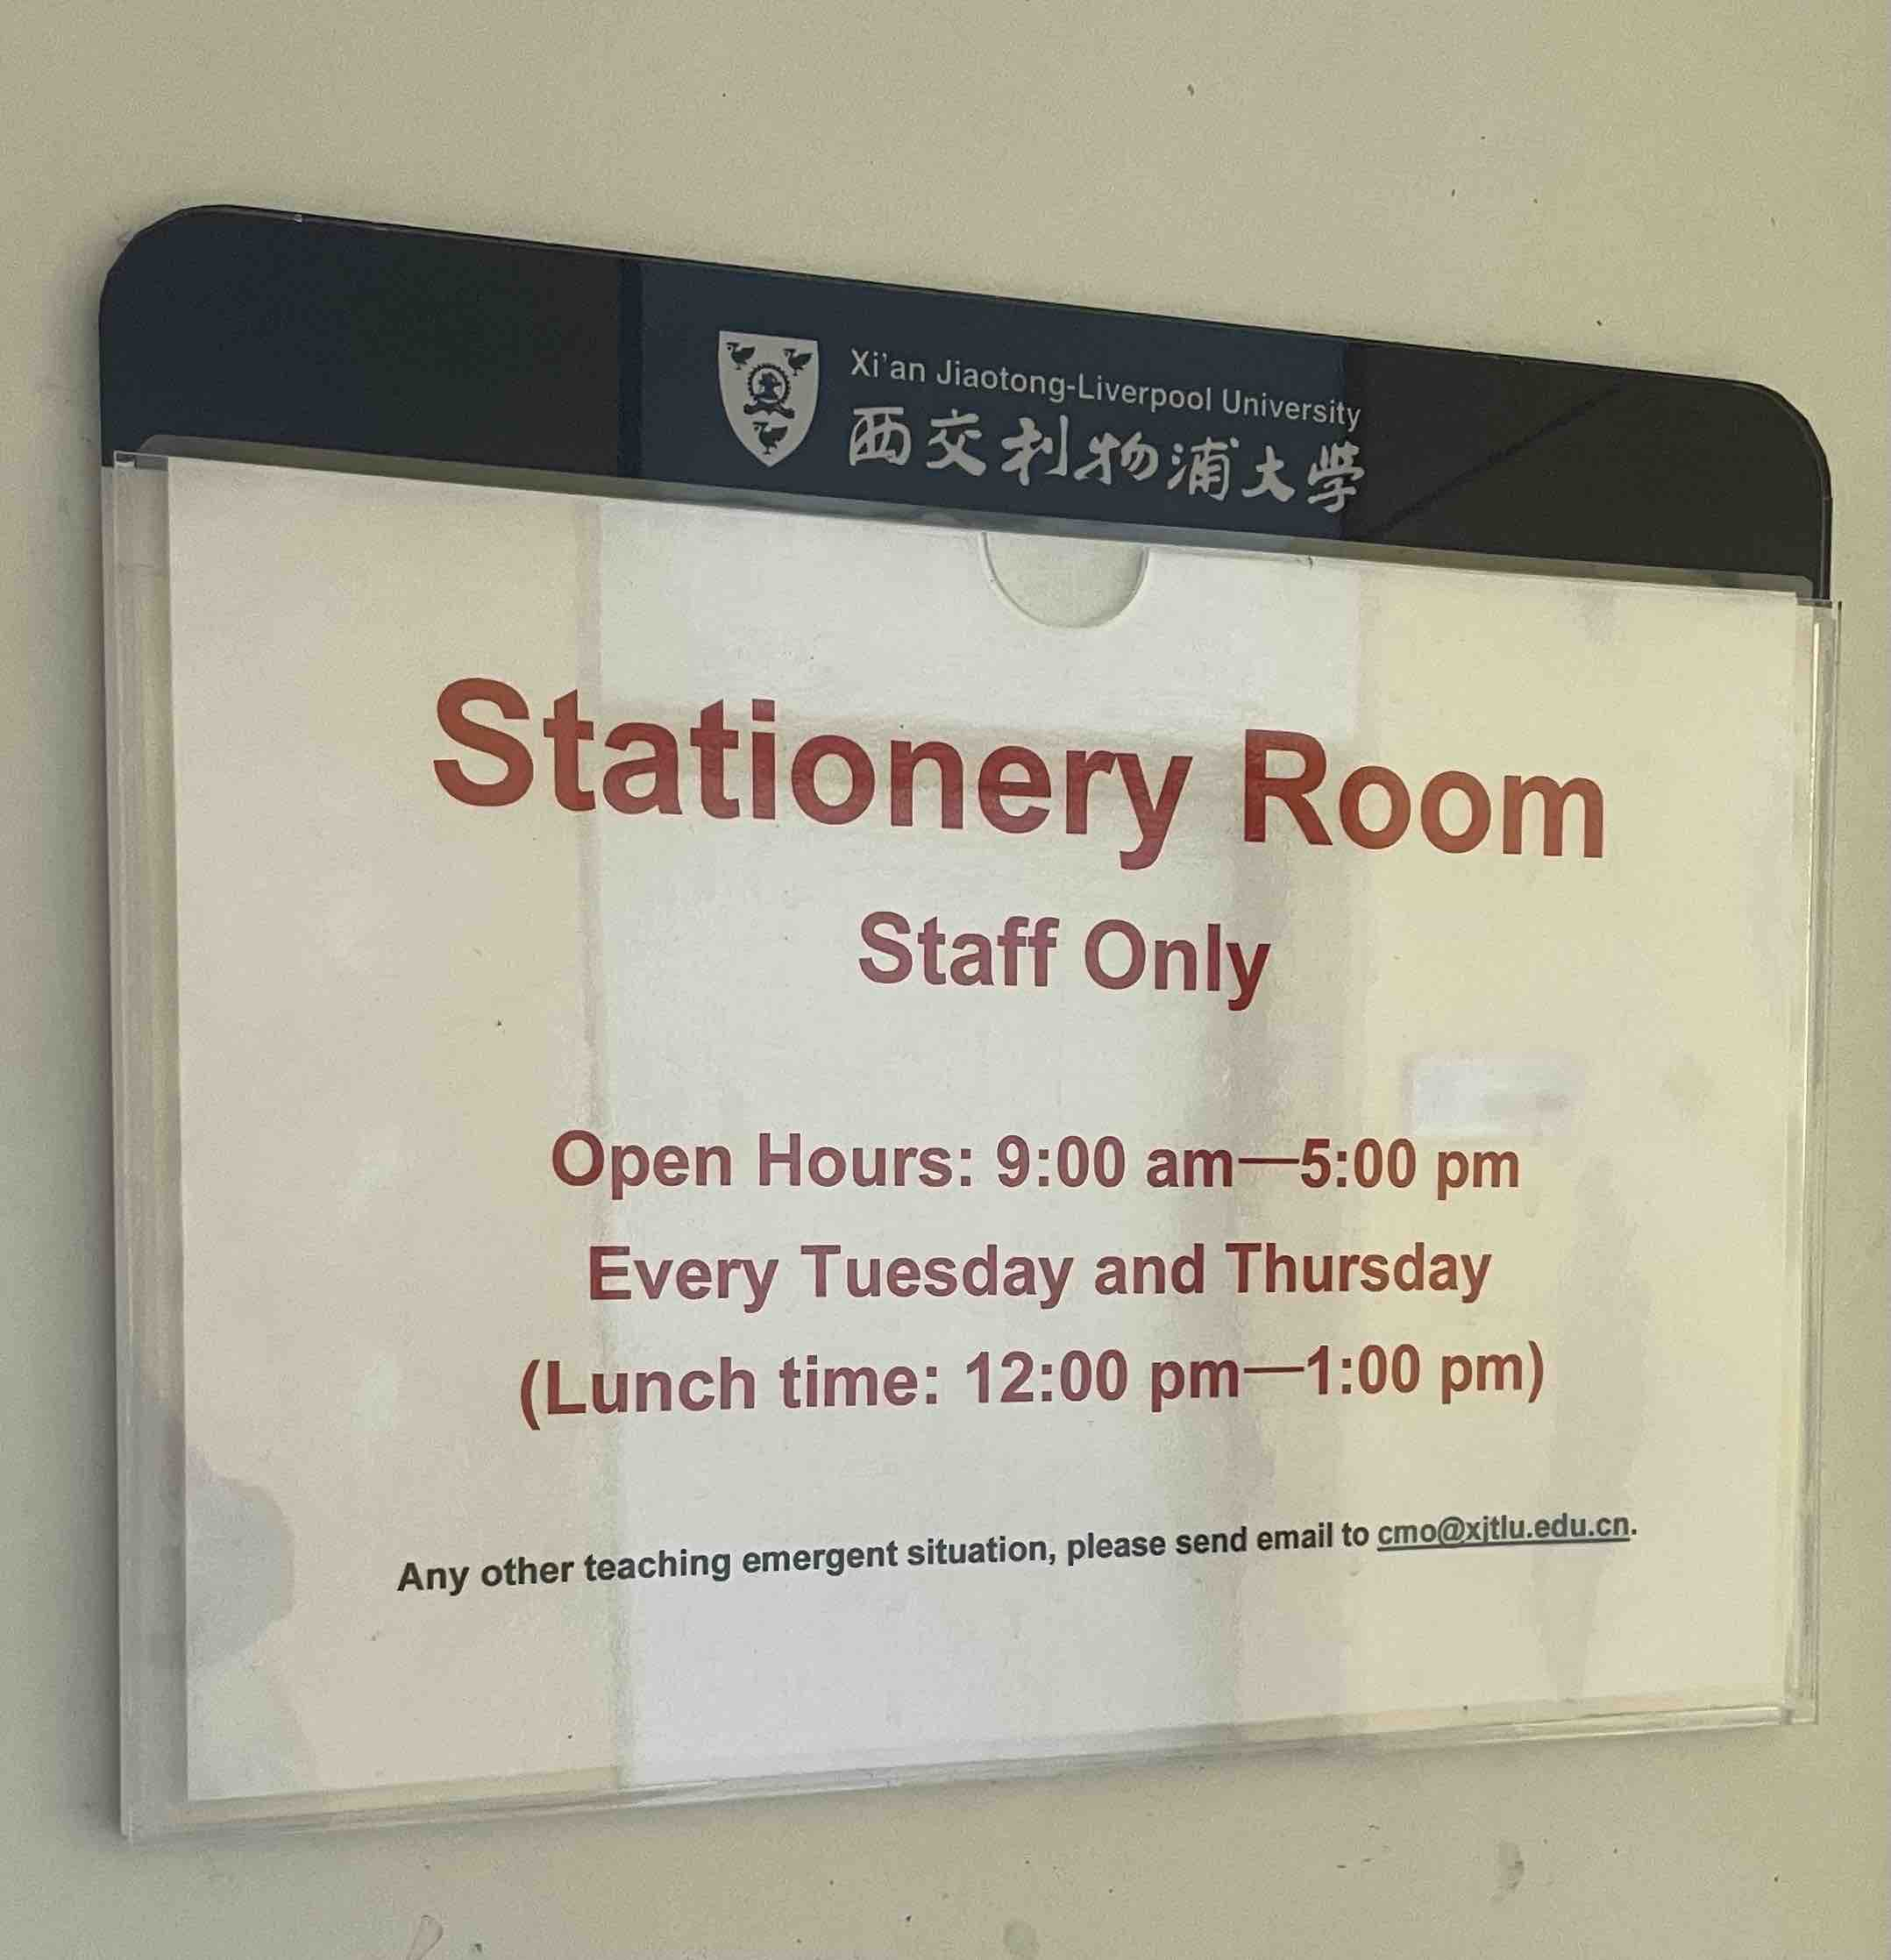
\includegraphics[width=0.6\columnwidth]{author-folder/Kai.Wu/stationery_room.jpg}
\end{figure}

除了大笔的会议经费之外,最让大家省钱的应该就是免费的办公用品了。学校很多楼里都有Stationery room(办公用品领用室),里面所有东西都可以领取。抽纸、笔、马克笔、荧光笔、各种收纳架子、胶带胶水订书机,基本你能想到的都有。

\vspace{5mm}
哪些地方有stationery room:
\begin{itemize}
    \item MB128,周二/周四,上午9-11点,下午1-5点
    \item BSG35,周二/周四,上午9-11点,下午1-5点(感谢匿名同学补充)
    \item HS楼物业,周一/三,上午9-11点,下午1-5点,周五上午(感谢匿名同学补充)
    \item 其他楼?请读者补充
\end{itemize}

\hfill\break
如何领取:
\begin{enumerate}
    \item 第一次领取前,先直接跑到stationery room,问工作人员可以领哪些,会给你一个册子。你直接拍照留存每一页内容,这样下次就知道可以拿什么了。或者,可以在这里找到一份热心同学上传的历史版本 \href{https://github.com/kaiwu-astro/xp_pgrs_unofficial_guide/tree/main/fileshare}{[GitHub链接]} \href{https://cowtransfer.com/s/ca761995ed6945}{[不能上GitHub的用这个链接]},但内容可能会变动而有少许差异。
    \item 下载最新的 (CMO) Office Supplies Application Form,目前最新版本是V3。新版本发布后老版本一般是不能用的。如果这个过期了,更新的版本我们在哪里下载呢?很遗憾我们没法下载\sout{(吐槽学校一次)},一般方法是,问你导师要,导师一般可以在学校的box网盘里面找到。这里提供一个我在用的 \url{https://cowtransfer.com/s/ca761995ed6945},也可在本项目的GitHub里(\href{https://github.com/kaiwu-astro/xp_pgrs_unofficial_guide/tree/main/fileshare}{链接})找到。
    \item 如实填写内容。其中第一列[办公用品名称]一定要和上面那个册子里的物品名称一样。每次不能拿太多,拿东西的工作人员会审查。抽纸每次只能拿一盒。笔一般是按支拿,不能按盒拿(但是你可以写拿12支,就是1盒)。右边的理由,如实简单填写,比如抽纸-日用;笔-演算;订书机-整理;胶水-报销。最后,要你导师签字。电子签名应该不能用,也不能导师签完过后复印(这些都是之前版本常用的花招hhh)。填完后,在stationery room开放时间拿过去,就可以愉快的free shopping啦。
    \item 202306更新:下面这些东西不用填表可以直接过去拿(其他的需要正常填表
\end{enumerate}

\begin{figure}[H]
    \centering
    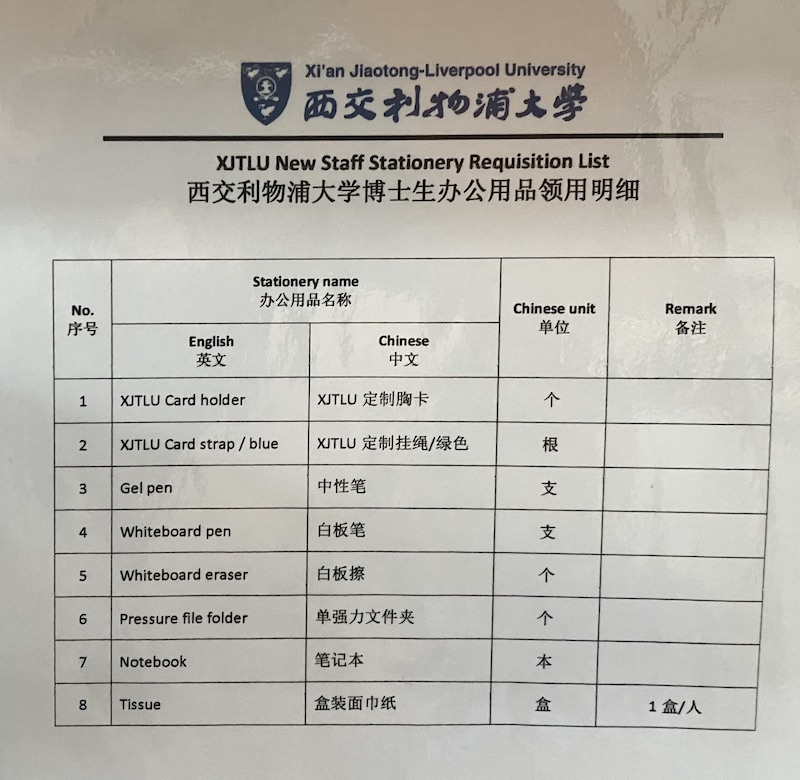
\includegraphics[width=0.6\columnwidth]{author-folder/Kai.Wu/stationery_no_sign.jpg}
\end{figure}


\begin{flushright}
(2022年10月12日 by Kai Wu)
\end{flushright}
